\section{METODOLOGIA}

\subsection{Modelaci\'on matem\'atica}

Tomando como base el m\'odulo de tres especies  IGP - \emph{depredaci\'on intragremial}-(descrito en \citealt{polis1989ecology,polis1992intraguild}),usamos un modelo matem\'atico \citep{holt1997theoretical} para describir las interacciones entre las especies componentes (recurso, consumidor intermedio(IG presa) y depredador tope(IG depredador) ). Este m\'odulo ha sido sugerido como un sistema de complejidad suficiente para incorporar distintos mecanimos que provocan variaci\'on en la longitud de las cadenas tr\'oficas : Inserci\'on, Adici\'on y Omnivorismo \citep{TP2007proximate}.

\subsubsection{Forma general}
La din\'amica del systema est\'a gobernada ,de forma general,por el siguiente sistema de ecuaciones diferenciales: \\
Sea $ N= (N_1,N_2,N_3) = (\dot{R} , \dot{C} , \dot{P}) : \mathbb{R}^3 \to \mathbb{R}^3 $
\begin{equation}\label{eq:Gsystem}
\begin{aligned}
&\dot{R} = F(R) -G(R,C)-H_{\R}(R,C,P)  \\
&\dot{C} = \epsilon_1 G(R,C)-H_{\C}(R,C,P) - q_2 C  \\
&\dot{P} = \epsilon_2 H_{\R}(R,C,P) +\epsilon_3 H_{\C}(R,C,P) -q_1 P
\end{aligned}
\end{equation}
\subsubsection*{Donde:}
\begin{tabular}{l@{:}p{5.8in}}
$R$\ &   Densidad de biomasa del recurso $R$.\\
$C$\ &  Densidad de biomasa del consumidor intermedio(IG prey) $C$.\\
$P$\ &  Densidad de biomasa del depredador tope(IG predator) $P$.\\
$F$\ &  Funci\'on que describe la din\'amica poblacional del recurso $R$ en ausencia de depredadores.\\
$G$\ &  Funci\'on que describe la depredaci\'on ejercida por el consumidor $C$ sobre el recurso $R$.\\
$H_{\R}$\ &  Funci\'on que describe la depredaci\'on ejercida por el depredador tope $P$ sobre el recurso $R$.\\
$H_{\C}$\ &  Funci\'on que describe la depredaci\'on ejercida por el depredador tope $P$ sobre el consumidor $C$.\\
$\epsilon_1$\ &  Eficiencia de conversi\'on de biomasa del recurso $R$ en biomasa del consumidor intermedio $C$.\\
$\epsilon_2$\ &  Eficiencia de conversi\'on de biomasa del recurso $R$ en biomasa del depredador tope $P$.\\
$\epsilon_3$\ &  Eficiencia de conversi\'on de biomasa del consumidor $C$ en biomasa del depredador tope $P$.\\
$q_1$\ &  Tasa de p\'erdida de biomasa por unidad de masa del consumidor intermedio $C$.\\
$q_2$\ &  Tasa de p\'erdida de biomasa por unidad de masa del depredador tope $P$.\\
\end{tabular}
\subsubsection{Forma espec\'ifica  \emph{Lotka-Volterra}}
En este caso asumimos que el recurso tiene un crecimiento log\'istico y que la tasa de consumo per c\'apita de biomasa escala linearmente con la densidad de biomasa del recurso, i.e., usamos una respuesta funcional Tipo I \citep{gotelliprimer}, la cual es una modificaci\'on del modelo Lotka-Volterra \citep{gotelliprimer}.\\
\mbox{}\\
Definimos:
\begin{equation}\label{eq:p1}
\begin{aligned}
&r := r(m_\R,T_\R,\vartheta_\R)&\\ 
&K := K(m_\R,T_\R,\vartheta_\R)&\\
&\alpha_{1} := \alpha_{1}(m_\R,m_\C,T_\R,T_\C,D_\R,f_1,\vartheta_\R,\vartheta_\C)&\\
&\alpha_{2} := \alpha_{2}(m_\R,m_\PP,T_\R,T_\PP,D_\R,f_2,\vartheta_\R,\vartheta_\PP)&\\
&\alpha_{3} := \alpha_{3}(m_\C,m_\PP,T_\C,T_\PP,D_\C,f_3,\vartheta_\C,\vartheta_\PP)& \\
&q_1 := q_1(m_\C,T_\C,\vartheta_\C)& \\ 
&q_2 := q_2(m_\P,T_\PP,\vartheta_\PP)&\\
&F(R):= rR(1-R/K)& \\
&G(R,C):= \alpha_1 RC &\\ 
&H_{\R}(R,C,P):= \alpha_2PR&\\
&H_{\C}(R,C,P):= \alpha_3PC&
\end{aligned}
\end{equation}

Reemplazando \eqref{eq:p1} en \eqref{eq:Gsystem} tenemos:

\
\begin{equation}
\begin{aligned} 
\dot{R} &= R\left[ r(1-\frac{R}{K})- \alpha_1 C -\alpha_2 P \right] \\
\dot{C} &= C \left[ \epsilon_1 \alpha_1 R - \alpha_3  P - q_1 \right] \\
\dot{P} &= P \left[ \epsilon_2 \alpha_2 R + \epsilon_3 \alpha_3 C - q_2 \right]
\end{aligned}
\end{equation}

\subsubsection*{Donde:}
\begin{tabular}{l@{:}p{5.8in}}
$r$  \ & Tasa intr\'inseca de producci\'on de biomasa del Recurso $R$.\\
$K$  \  &Capacidad de carga (en biomasa) del recurso $R$.\\
$\alpha_1$  \ & Tasa por unidad de masa de b\'usqueda y captura de biomasa del depredador intermedio $C$ sobre  el recurso basal $R$.\\
$\alpha_2$ \ & Tasa por unidad de masa  de b\'usqueda y captura de biomasa del depredador tope $P$ sobre  el recurso basal $R$.\\
$\alpha_3$ \  &Tasa por unidad de masa de b\'usqueda y captura de biomasa del depredador tope $P$ sobre  el depredador intermedio $C$.\\
$m_\R$  \ & Masa de un individuo ``t\'ipico'' del recurso $R$.\\
$m_\C$  \ & Masa de un individuo ``t\'ipico'' del consumidor intermedio $C$.\\
$m_\textit{\tiny P}$  \ & masa de un individuo ``t\'ipico'' del depredador tope $P$.\\
$T_J$ \ & Temperatura corporal promedio de la especie $J$, donde $J$ puede ser: $P,C,R$ \\
$\vartheta_J$ \ & Clase metab\'olica de la especie $J$, donde $J$ puede ser: $P,C,R$ \\
$D_J$  \ & Dimensi\'on del espacio en el cual se desarrola depredaci\'on sobre la presa $J$, donde $J$ puede ser: $R$ o $C$.\\
$f_1$ \ & Estrategia de forrajeo de la consumidor intermedio $C$ .\\
$f_2$ \ & Estrategia de forrajeo del depredador tope $P$ sobre $R$ .\\
$f_3$ \ & Estrategia de forrajeo del depredador tope $P$ sobre $C$ .\\
\end{tabular}

Los par\'ametros y funciones no mencionados mantienen la descripci\'on dada en el caso general.
\subsubsection{Parametrizaci\'on}
Usamos relaciones alom\'etricas derivadas previamente en la literatura basadas en relaciones biomec\'anicas y bioenerg\'eticas \citep{savage2004predominance,brown2004toward,west1997general,savage2004effects,pawar2012dimensionality,mcgill2006allometric,peters1986ecological,kiltie2000scaling,yodzis1992body} para exponer expl\'icitamente la variaci\'on de los par\'ametros de los modelos usados con respecto a la masa corporal de las especies interactuantes,  si bien la temperatura se puede incluir expl\'icitamente en estas relaciones (v\'ease \citealt{brown2004toward,savage2004effects}) nos centraremos \'unicamente en la masa corporal y dejaremos los efectos de la temperatura para un futuro trabajo.

\subsubsection{Par\'ametros intra-poblacionales}
Usando las relaciones definidas en \cite{savage2004effects} tenemos:
\begin{equation}\label{eq:params3}
\begin{aligned}
&r = r_0m_\R^{\beta_\R - 1} \\
&q_1=q_{0,1}m_\C^{\beta_\C - 1} \\
&q_2= q_{0,2}m_\PP^{\beta_\PP -1}\\
&K= K_{0}m_\R^{1-\beta_\R}
\end{aligned}
\end{equation}

$\beta_J$ es el exponente que describe la variaci\'on de la tasa metab\'olica a nivel de individuo con la masa de la especie $J$, cuyo valor ha sido descrito entre $2/3 - 1$ siendo $3/4$ el asociado a una tasa metab\'olica basal y valores superiores a tasas metab\'olicas en actividad\citep{pawar2012dimensionality,west1997general,savage2004predominance}. \\
$r_0,q_{0,1},q_{0,2}$ y $K_0$ son constantes que dependen de la temperatura y la clase metab\'olica de las especies( e.g., endotermos o ectotermos) , $K_0$ a su ves depende de la productividad del ecosistema \citep{pawar2012dimensionality}.
\subsubsection{Par\'amatros inter-poblacionales}
Usando las relaciones definidas en \citep{pawar2012dimensionality,kiltie2000scaling,mcgill2006allometric,bejan2006unifying} tenemos una relaci\'on para $m_j\alpha$  la tasa p\'ercapita de b\'usqueda(tasa de encuentro potencial) y captura de biomasa de recurso $i$ por parte de un depredador $j$, la cual depende del \'area buscada $S_A$ y la tasa de \'exito en la captura $\aleph$ : 

\begin{equation}\label{eq:alfa}
\begin{aligned}
 m_j\alpha & =  S_A*\aleph \\
 S_A &=  A_D * v_r \\
A_D &=  \begin{cases} 2d & \text{si } D_i = 2 \\ \pi d^2 & \text{si } D_i = 3 \end{cases}\\
v_r &= \sqrt{v_i^2 +v_j^2}\\
\aleph &= \Pi(k_{ij})
\end{aligned}
\end{equation}
A continuaci\'on detallamos cada componente de \eqref{eq:alfa}:\\

$A_D$ se deriva del hecho que el la regi\'on de detecci\'on del depredador $j$ es una ($D_i-1$)-esfera independientemente de la forma de detecci\'on\citep{pawar2012dimensionality}.Donde $D_i$ es la dimensi\'on en la cual se desarrolla la interacci\'on la cual esta determinada por la dimensi\'on del espacio en el cual se distribuye el recurso $i$.\\
$v_r$ es la velocidad relativa presente entre $i$ y $j$ , que se interpreta como el promedio poblacional de la rapidez con la cual convergen $i$ y $j$ en el h\'abitat \citep[supinfo.]{pawar2012dimensionality} , la forma dada en \eqref{eq:alfa} asume un movimiento aleatorio por parte de ambas especies, el cual ha sido descrito previamente \citep{okubo2001diffusion}.\\
En \cite{pawar2012dimensionality} describen la variaci\'on de la velocidad para una especie $v$ respecto a cambios en su masa corporal de la siguiente manera:
\begin{equation}\label{eq:vel}
\begin{aligned}
&v \propto \frac{B_0 m^\beta}{Fuerza}\\
&Fuerza \propto m^{\beta_F} \\
&v = v_0m^{\beta - \beta_F}
\end{aligned}
\end{equation}
$v_0$ es una constante que depende de la taxa y del modo de locomoci\'on y la constante metab\'olica $B_0$.\\

$k_{ij}= m_i/m_j$ es el raz\'on de la masa del recurso con respecto al depredador , y $\Pi \in [0,1]$ y  puede tomar distintas formas\citep{weitz2006size}, en este trabajo se us\'o la siguiente(figura \ref{fig:efficiency}): 
\begin{equation}\label{eq:sr}
\Pi(k_{ij}) =\frac{a}{1+k_{ij}^\phi} \\
\end{equation}

$a \in [0,1] $ es una constante que determina la m\'axima eficiencia en la captura y $\phi > 0 $ determina la forma del decaimiento de $\Pi$ con respecto a $k_{ij}$, notar que $\lim_{k_{ij} \to +\infty}  \Pi(k_{ij}) = 0$ y  $\lim_{k_{ij} \to 0} \Pi(k_{ij}) = a $.

\begin{figure}
\begin{center}
 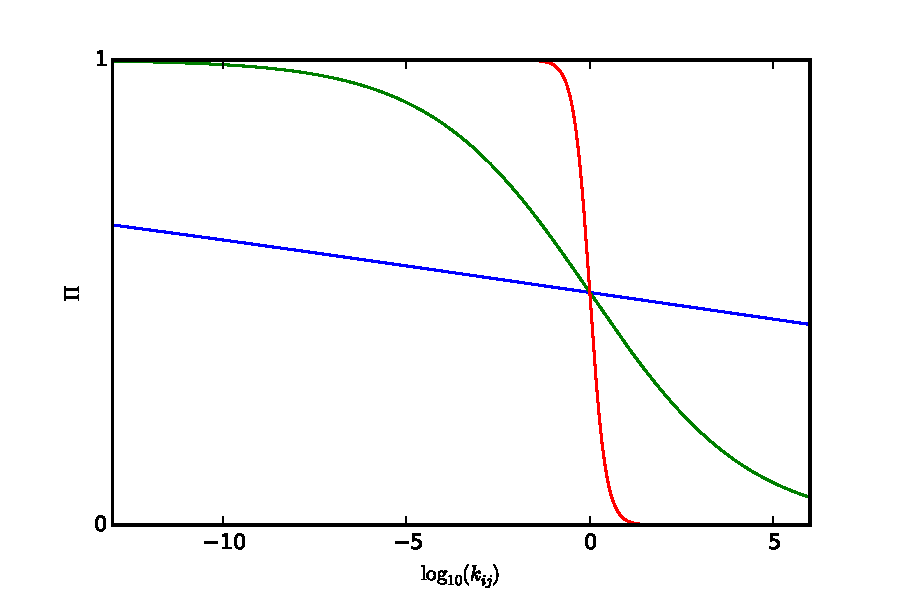
\includegraphics[width=0.7\textwidth]{./Plots/CaptureEfficiency.pdf}
 \caption[$\Pi$]{ Formas para $\Pi$ en escala logar\'itmica para distintos valores de $\phi$ , ({\hwplotB}) = 0.02 , ({\hwplotG}) = 0.2 y ({\hwplotR}) = 2 . Donde se observa que si $\phi_1 > \phi_2$ entonces $\Pi_{\phi_1}(k_{ij}) >\Pi_{\phi_2}(k_{ij})$ para $k_{ij} < 1$ y lo contrario en caso $k_{ij}>1$ }
 \label{fig:efficiency} 
\end{center}
\end{figure}

$d$ es el radio de detecci\'on m\'aximo a la cual un depredador de un tama\~no percibe a la presa, la relaci\'on con el tama\~no corporal se desprende del siguiente argumento:\\ Sea $\eta$ la agudeza visual del depredador $j$ y $\theta$ el \'angulo de resoluci\'on:
\begin{equation}\label{eq:d}
\begin{aligned}
\tan{\theta/2} &= \frac{L_{j}}{d} \\
\theta &= \frac{1}{\eta} \\
\eta & = c_a L_i^{b_a} \\
M &= c_{lm}L^{b_{lm}} 
\end{aligned}
\end{equation}
\subsubsection*{Donde:}
$L_i , L_j$ son las longitudes corporales del recurso $i$ y depredador $j$ respectivamente. \\La \'ultima relaci\'on expresa la alometr\'ia existente entre la longitud y la masa de una espacie, $b_{lm} \approx 3 $ y $c_{lm}$ es una constante que depende de la forma y densidad de la especie \citep{peters1986ecological,mcgill2006allometric}. \\
$b_a \approx 1 $ y $c_a$ varia dependiendo del grupo taxon\'omico y el ambiente \citep{kiltie2000scaling} .\\
\cite{pawar2012dimensionality} derivan $d$ de la siguiente relaci\'on:
\[ d = d_0(m_im_j)^{p_d} \]
La cual es una aproximaci\'on plausible derivada de \eqref{eq:d} y es la que nostros usamos. $d_0$ y $p_d$ son constantes que son influenciadas por la dimensi\'on del espacio de b\'usqueda $D$. \\
Realizando algunas simplificaciones en \eqref{eq:alfa} se llega a obtener la siguiente forma para la respectiva tasa de ataque $\alpha$ \citep{pawar2012dimensionality}.

\begin{equation}\label{eq:p4}
\begin{aligned}
&m_\C \alpha_1= \alpha_{0,1}m_\C^{p_v+2p_d(D_R-1)}f_1(k_{\RC})\\
&m_\PP \alpha_2= \alpha_{0,2}m_\PP^{p_v+2p_d(D_R-1)}f_2(k_{\RP})\\
&m_\PP \alpha_3= \alpha_{0,3} m_\PP^{p_v+2p_d(D_C-1)}f_3(k_{\CP})\\
\end{aligned}
\end{equation}
\subsubsection*{Donde:}
$p_v$ y $p_d$ son exponentes que controlan como escala la velocidad de un individuo  y la distancia de reacci\'on con el tama\~no corporal, respectivamente. El valor de $p_d$ var\'ia ligeramente con la dimensi\'on en la cual se desarrolla la interacci\'on \citep{pawar2012dimensionality}.\\
La funci\'on $f$ incorpora tanto los cambios sobre $S_A$ como $\aleph$ respecto a $k$ y a su vez es dependiente de la estrategia de forrajeo($Fm$) del depredador donde tres casos son considerados\citep{pawar2012dimensionality}.
\begin{itemize}
\item Captura activa ($Ac$).
\item Pastoreo ($Gr$).
\item Captura pasiva-\textit{Sit and wait}.($Sw$) 
\end{itemize}

\begin{equation}\label{eq:fkr}
f(k_{ij}) = 
\begin{cases}
\sqrt{1+k_{ij}^{2p_v}}k_{ij}^{(D_j-1)p_d} \Pi(k_{ij}) & Fm = Ac\\
k_{ij}^{p_v+(D_j-1)p_d}\Pi(k_{ij}) & Fm =Gr\\
k_{ij}^{(D_j-1)p_d}\Pi(k_{ij}) & Fm = Sw\\
\end{cases}
\end{equation}

Un an\'alisis del comportamiento de estas funciones se detalla en anexos \ref{subsec:funcf}.


\subsection{An\'alisis}
Todos los an\'alisis descritos a continuaci\'on se desarrollar\'an para el modelo descrito y con distintas combinaciones de dimensi\'on del habitat, estrategia de forrajeo,nivel de productividad ambiental basal y $\Pi$, las combinaciones usadas se especifican en Anexo \ref{subsec:params} .\\
Definiendo:
\begin{equation}
  k_\RC = \frac{ m_R}{m_C} \ \ \land k_\CP = \frac{m_C}{m_P}
\end{equation}
Como la \emph{raz\'on de masas presa-depredador},podemos expresar $m_R$ y $m_C$ en funci\'on a $m_P$ y la respectiva raz\'on de masas, esto sumado a la parametrizaci\'on empleada nos sirve para explorar los efectos que causan estos 3 par\'ametros sobre las propiedades del m\'odulo. Fijando las dem\'as constantes reducimos el espacio param\'etrico se reduce a tres ejes : $k_\RC,k_\CP, m_p$(note que $k_\RP = k_\RC k_\CP$). \\
A su vez se debe notar que aumentos en $m_P$ para un par de $k_\RC$ y $k_\CP$ fijos, aumentan la masa de las tres especies. 

\subsubsection{Criterios de Invasibilidad}\label{subsubsec:Inv}
Se delimitaron zonas dentro del espacio param\'etrico donde era posible la invasi\'on de una de las especies sobre un sistema receptor(debido a esto se les denomina \emph{criterios de invasibilidad}), para el sistema que estamos analizando los siguientes escenarios son posibles: 

\begin{itemize}
\item $R$ invade un sistema \emph{vac\'io}.
\item $C$ invade un sistema conformado solo por $R$.
\item $P$ invade un sistema conformado solo por $R$.
\item $P$ invade un sistema conformado por $R$ y $C$.
\item $C$ invade un sistema conformado por $R$ y $P$.
\end{itemize}
En los 3 primeros escenarios la variaci\'on de la longitud de la cadena tr\'ofica involucra al mecanismo de \textit{adici\'on} y en el \'ultimo escenario el mecanismo involucrado es el de \textit{inserci\'on}.\\

La derivaci\'on de estos criterios asume lo siguiente:
\begin{itemize}
\item \emph{El sistema receptor se ha encontrado aislado por suficiente tiempo como para alcanzar un estado asimpt\'otico y que dicho estado es un punto de equilibrio}.\\Esta suposici\'on es plausible ya que se espera que los eventos de inmigraci\'on de $C$ y $P$ no coincidan y que la separaci\'on entre ambos sea \emph{suficientemente} larga. M\'as a\'un en el modelo usado, en cualquier subsistema de dos especies(e.g $R-C$) la condición inicial (e.g. $(R_0,C_0) \in R_2^+$) pertenece al dominio de atracci\'on del punto de equilibrio.(Un simple an\'alisis gr\'afico del plano de fases da ese resultado \citep{gotelliprimer}).
\item \emph{La invasi\'on se considera exitosa si es que existe un crecimiento por parte del invasor en los instantes posteriores a la invasi\'on}. *En el caso del sistema tridimensional esta condición es necesaria para la invasión.
\end{itemize}

Se calcularon 5 criterios de invasibilidad $\mathbf{I_{\R},I_{\C \to \R},I_{\PP \to \R},I_{\PP \to \C-\R},I_{\C \to \PP-\R}}$ y se asoci\'o a cada uno la zona del espacio param\'etrico explorado donde se cumplen, la zona asociada al criterio $I$ se denota por $\mathbf{Z(I)}$ .\\

Un ejemplo de la forma de calcular estos criterios se detalla a continuaci\'on, y los dem\'as se especifican en \ref{subsec:CI}

\myparagraph{P $\to$ C-R}

\begin{equation} \mathbf{IC_{\PP \to \C-\R}} := \dot{P} >0 \iff \epsilon_2\alpha_2\hat{R}_2 + \epsilon_3\alpha_3\hat{C}_2 > q_2 m_P \end{equation}

Donde:
\begin{equation}
\begin{aligned}
\hat{R}_2 &= \frac{q_1 m_C}{\epsilon_1 \alpha_1} \\
\hat{C}_2 &=  r(\frac{m_C}{\alpha_1}) \left[ 1 - \frac{q_1 m_C}{\epsilon_1 \alpha_1 K} \right] 
\end{aligned}
\end{equation}

\begin{equation}
\mathbf{Z(I_{\PP \to \C-\R})} := \{ v \in \mathbf{Z(I_{\C \to \R})} / \dot{P}(v) > 0 \}
\end{equation}


\subsubsection{Zonas de Coexistencia}
Se delimitaron zonas dentro del espacio param\'etrico donde el triple equilibrio $\mathbf{X} = (R^*,C^*,P^*)$ fuese positivo, $\mathbf{X}$ tiene la propiedad de que $N(\mathbf{X}) = 0$ para $N$ descrito en \eqref{eq:Gsystem}. El conjunto de los puntos de equilibrio es denotado por $E$.
\begin{equation}\label{eq:Equilibrio}
E:= \{ (R,C,P) \in \mathbf{R}^3_+ / N((R,C,P)) = 0 \}
\end{equation}

En nuestro caso las expresiones para el equilibrio son(el c\'alculo se detalla en \ref{subsec:equil}):
\begin{flalign}
R^* &= \frac{K(\epsilon_3 ( \alpha_2 q_1 + \alpha_3 r) - \alpha_1 q_2)}{A}& \\
C^* &= \frac{K\alpha_1 \alpha_2 \epsilon_1 q_2 - K \alpha_2 \epsilon_2 ( \alpha_2 q_1 + \alpha_3 r) + \alpha_3 q_2 r} {\alpha_3 A} \\
P^* &= \frac{K \alpha_1 (\alpha_2 \epsilon_2 q_1 + \alpha_3 \epsilon_1 \epsilon_3 r) - (K \alpha_1^2 \epsilon_1 q_2 + \alpha_3 \epsilon_3  q_1 r)}{\alpha_3 A }
\end{flalign}
Donde:
\begin{equation}
A = K \alpha_1 \alpha_2 (\epsilon_1 \epsilon_3 - \epsilon_2 ) + \alpha_3 \epsilon_3 r
\end{equation}
Manipulando algebraicamente $C^*$ y $P^*$ se deriva que la condici\'on para que $(R^*,C^*,P^*)$ pertenzca a $R^3_+$ es que se cumplan $I_{\C \to \PP-\R}$ y $I_{\PP \to \C-\R}$ en el caso que $A >0$ y que no se cumplan ambos en caso que $A<0$. Si $A = 0$ el sistema no posee equilibrio no trivial. \\
Dado lo descrito anteriormente en el caso que $A <0$ el equilibrio no puede formarse mediante ning\'un camino de ensamblaje con los supuestos hechos en \ref{subsubsec:Inv}.\\
 Denotamos :
\begin{equation}
  \begin{aligned}
    E_1 &= \{ n \in E / A >0 \}  \\
    E_2 &= \{ n \in E / A <0 \}
  \end{aligned}
\end{equation}

\myparagraph{Habilidad Competitiva}
Se puede derivar que una condici\'on necesaria para que el sistema tenga un equilibrio estable es la siguiente:
\begin{equation}
  \frac{q_2}{\varepsilon_2 \alpha_2 } > \frac{q_1}{\varepsilon_1 \alpha_1}
\end{equation}
Lo cual es equivalente a que $R^*_\PP < R^*_\C$ que denota una mayor habilidad competitiva por parte del consumidor intermedio seg\'un la \emph{regla R}\citep{Tilman1990}.

Con la parametrizaci\'on usada para una masa de depredador tope $m_P$ dada esta condici\'on se reduce a 
\begin{equation}
  \frac{q_{0,2}}{\varepsilon_2 \alpha_{0,2} f_2(k_{\RP})} > \frac{q_{0,1} k_{\CP}^{\beta-h}}{\varepsilon_{1} \alpha_{0,1} f_1(k_{\RC})}
\end{equation}

Donde $ h = p_v + 2(D_R -1) p_d$.

\subsubsection{Estabilidad Din\'amica}
En cada regi\'on de coexistencia se distingui\'o entre puntos \emph{localmente estables e inestables},el procedimiento se detalla en \ref{subsec:stab},y se determin\'o la influencia sobre:
\begin{equation}\label{eq:estabreg}
E_{estab} = \{ (R,C,P) \in E / (R,C,P) \mbox{ es localmente estable} \}
\end{equation}

